\chapter{Implementacion Digital} \chapterlabel{Informe/7-ImplementacionDigital} \label{cap:Implementacion Digital}

\section{Descripción general}

\noindent La implementación digital consiste, básicamente, en realizar la estimación de posición y el control de la planta por medio de un microcontrolador. Se utiliza un kit de desarrollo basado en el microcontrolador STM32F072, que contiene un ADC de 12 bits y 3.3V de referencia, un DAC 12 bits y 3.3V de referencia.

\noindent En la figura \ref{fig:diag-en-bloques-digital} se muestra un diagrama en bloques general de la implementación digital del sistema. Es posible observar que se ingresa al microcontrolador a través de un ADC, con una tensión de referencia ($V_{ref}$) proporcional a la distancia de separación deseada. Esa posición de referencia es comparada con la posición estimada Y(z) y el resultado e(z) es afectado por el compensador digital C(z). Por medio de un DAC, la salida del compensador ingresa al controlador de corriente $G_{iL}(s)$, el cual actúa sobre la planta $G_P(s)$, modificando así la distancia de separación.

\noindent Por medio de un ADC y el sensor de Efecto Hall, se muestrea una tensión proporcional a la corriente que circula por el electroimán. De esta forma, es posible obtener una posición estimada Y(z) al multiplicar esta tensión por la transferencia H(Z).


\begin{figure}[H]
	\centering
	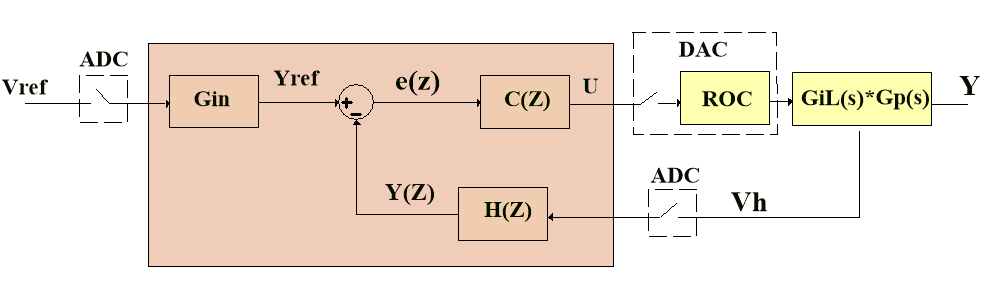
\includegraphics[scale=0.5]{Diagrama-en-bloques-digital.png}
	\caption{Diagrama en bloques de la implementación digital.}
	\label{fig:diag-en-bloques-digital}
\end{figure}

\noindent Abstrayéndose de la matemática que se realiza dentro del micro para la estimación de posición, podemos simplificar el diagrama al que se muestra en la figura \ref{fig:diag-en-bloques-digital-simplif}, en la que:

\begin{equation} 
	G_T(s) = G_P(s) * G_{iL}(s).
\end{equation}

\begin{figure}[H]
	\centering
	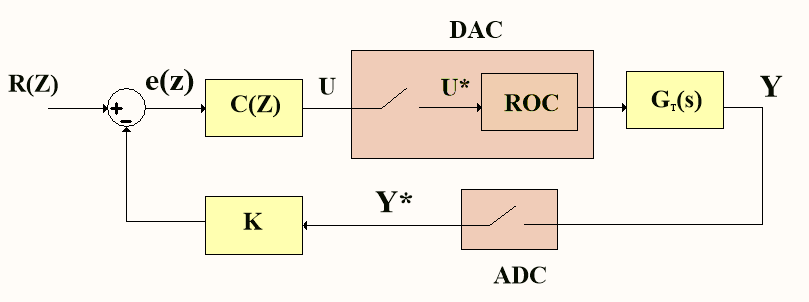
\includegraphics[scale=0.5]{Diagrama-en-bloques-digital-simplificado.png}
	\caption{Diagrama en bloques de la etapa digital simplificado.}
	\label{fig:diag-en-bloques-digital-simplif}
\end{figure}


\section{Determinación de la frecuencia de muestreo}

\noindent Se desea realizar una estimación de la posición del electroimán Y(z)  a partir de las muestras tomadas por el ADC de la tensión de salida del sensor de efecto HALL.

\noindent La forma de onda de la salida del sensor es triangular y presenta una frecuencia variable en función de la inductancia del electroimán, la que, depende de la distancia de separación. Se puede calcular como:

\begin{equation} 
	F_{SW}=\frac{V_{BUS}}{2 * L(y) * \Delta I_H}
\end{equation}

\noindent Dadas las mediciones realizadas sobre el electroimán, se obtuvieron los valores de inductancia al variar la distancia de separación del entrehierro. Al aplicar en la ecuación 5.1 los valores de inductancia obtenidos en la medición (L[mHy]), se calcula la frecuencia de conmutación  $(F_{SW}[Hz])$. Los resultados se muestran en la tabla \ref{frecuencias-calculadas}.


\begin{table}[H]
	\begin{center}
		\begin{tabular}{| c | c | c |}
			\hline
			Y[mm] & L[mHy] & $F_{SW}[Hz]$\\ \hline
			2 & 22.64 & 1060\\ \hline
			3 & 18.8 & 1276\\ \hline
			4.4 & 15.5 & 1548\\ \hline
			5.2 & 14.7 & 1632\\ \hline		
			6.5 & 14.4 & 1666\\ \hline
		\end{tabular}
		\caption{Valores de frecuencia calculados a partir de las mediciones de inductancia realizadas.}
		\label{frecuencias-calculadas}
	\end{center}
\end{table}


\noindent Para la estimación de la posición es necesario medir la pendiente de la onda triangular. Por lo que, para reconstruir su forma de onda es necesario muestrear la señal con cierta cantidad de armónicos para no afectar demasiado la pendiente. Se determinó que la frecuencia de muestreo del ADC debe ser al menos el doble de la frecuencia de la 5º armónica para el caso de la mayor frecuencia. Por lo tanto, se adopta 2.5 veces. Es decir:


\begin{equation} 
	F_S \geq 2.5 * 5 * f_{max} \Rightarrow  F_S \geq 2.5 * 5 * 1666 Hz \Rightarrow F_S \geq 20825 Hz
\end{equation}

\noindent De esta forma, se adopta una frecuencia de muestreo para el ADC de  25 kHz. Por lo tanto, es posible obtener 15 muestras en un período de la triangular para el caso de la frecuencia máxima. Como la señal crece o decrece durante medio ciclo, se pueden tomar 7 muestras para identificar la pendiente. En el caso de que la señal presente la frecuencia mínima, se pueden tomar 23 muestras en un ciclo, lo cual se traduce en 11 muestras para la pendiente de subida o bajada. 


\section{Adquisición y procesamiento de las muestras}

\noindent Considerando el caso de máxima frecuencia, en el que solo se podrán tomar 7 muestras durante el tiempo de crecimiento o decrecimiento, se describe el procedimiento para determinar la posición estimada.


\begin{figure}[H]
	\centering
	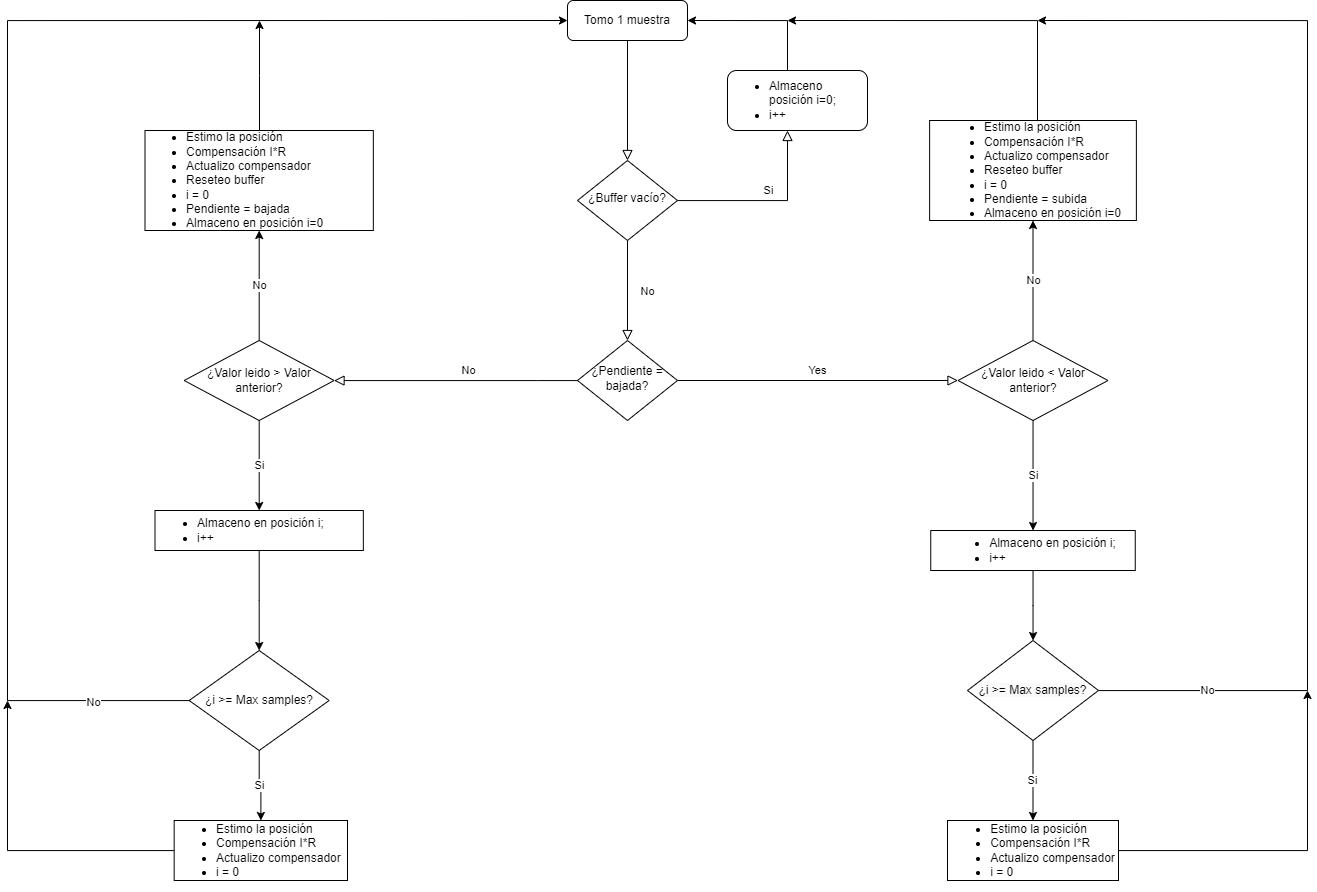
\includegraphics[scale=0.3]{Procesamiento-muestras-adquiridas.png}
	\caption{ Diagrama de flujo del procesamiento de las muestras adquiridas.}
	\label{fig:procesamiento-muestras-adquiridas}
\end{figure}


\noindent Como se observa en el diagrama de flujo de la figura \ref{fig:procesamiento-muestras-adquiridas}, cada muestra de tensión tomada del sensor de efecto hall, se almacena en un buffer de 7 posiciones. Para poder discernir entre pendientes de bajada y de subida, se verifica en cada muestra si el valor leído es mayor o menor al almacenado en la posición anterior. En caso de que sea mayor al anterior, significa que se está muestreando la pendiente positiva de la onda triangular. El hecho de poder discernir entre pendientes positivas y negativas, permite aplicar la compensación I*R al igual que se realiza en el estimador analógico. 

\noindent Cada vez que el buffer se complete, se realiza el cálculo de la derivada con el valor máximo y mínimo almacenado. Con este resultado, se hace la estimación de la posición y se actualiza la entrada al compensador digital.

\noindent En caso de haber completado las 7 posiciones del buffer y la pendiente persiste con el mismo signo, el buffer comienza a llenarse nuevamente desde la posición inicial, sobreescribiendo los valores de mayor vejez. Por lo tanto, pueden ocurrir dos situaciones. La primera es que se detecte un cambio de pendiente antes de completar nuevamente el buffer, con lo cual se calcula la derivada con los valores extremos almacenados sin importar su vejez y se actualiza la entrada al compensador. La segunda, es que se vuelva a completar el buffer, en cuyo caso también se hace la actualización. La diferencia entre estas dos situaciones es el tiempo transcurrido. En este último, se hace cada 7 períodos de muestreo mientras que en el primero se realiza “N” períodos de muestreo luego de la última actualización, donde “N” representa la cantidad de muestras que se almacenaron en el buffer incompleto.

\noindent Luego de cada actualización, el proceso vuelve a iniciar con el buffer vacío.

\noindent Utilizando este método de estimación, puede ocurrir que se obtenga una nueva estimación en 7 periodos de muestreo del ADC, o incluso en menos. Por lo tanto se podría decir que se tiene un estimador de posición con frecuencia de actualización variable. Esto es importante al momento de diseñar un compensador digital para el sistema. Para hacerlo, se debe considerar el caso en que la frecuencia de actualización es la menor, por lo tanto podríamos decir que el compensador digital se debe diseñar con una frecuencia de muestreo de 25/7 KHz = 3.5 KHz.

\section{Estimación digital de la posición}

\noindent De las mediciones realizadas se llegó a la expresión que relaciona la distancia de separación con la pendiente de la corriente en el electroimán:

\begin{equation} 
	|\frac{di_L}{dt}[A/s]| = 194690 * Y[m] + 676 [A/s]
\end{equation}

\noindent Por lo tanto, la posición en metros puede despejarse como:

\begin{equation} 
	Y = 5.136*10^{-6}*|\frac{di_L}{dt}|- 3.472*10^{-3} [m]
\end{equation}

\noindent Es importante notar que la resistencia interna (R) del electroimán genera una caída de tensión cuando circula corriente. Esta caída provoca que la tensión efectiva aplicada sobre la inductancia sea distinta para el semiciclo de subida que el de bajada, generando que la onda triangular tenga diferentes pendientes (en valor absoluto) para cada caso. Esta se representa como $(\frac{di_L}{dt})_{Real}$ y es la que se mide al utilizar el ADC.

\noindent Es decir:

\begin{equation} 
	(\frac{di_L}{dt})_{Real}=(\frac{di_L}{dt})_{Teorica}-\frac{R*I_L}{L(y)}
\end{equation}

\noindent Aproximando la derivada real como la resta entre la muestra en un instante menos el anterior sobre el período de muestreo y compensando el error que introduce la resistencia interna, se obtiene:

\begin{equation} 
	Y = 5.136*10^{-6}* |\frac{I_L[n]-I_L[n-1]}{T_S}+\frac{R*i_L}{L(y)}| - 3.472*10^{-3} [m]
\end{equation}


\noindent Considerando a $V_h$ como la tensión entregada por el sensor de efecto hall, proporcional a la corriente que circula por el electroimán multiplicada por una ganancia $K_h$ de 53.3mV/A, donde  ($\hat{V_h}$)  corresponde a la componente alterna de tensión y ($\bar{V_h}$) la continua, resulta:


\begin{equation} 
	V_h[n] = \bar{V_h}[n] + \hat{V_h}[n] = K_h * (\bar{I_L}[n] + \hat{I_L}[n])
\end{equation}

\noindent Para la estimación de la posición se utiliza el término de alterna mientras que para compensar el error introducido por la resistencia interna del electroimán se utiliza el de continua. Por lo tanto, se obtiene:





